\documentclass{article}

\usepackage{GSReg-style}

\title{GlobalSearchRegression.jl \\
       \vspace{5mm} REPORT} 

%\author{
%  Insert author name \\
%  Insert Institution/Affiliation \\
%  Insert other researcher information \\
%  \texttt{insert@email.com} \\
%   \and if there are more authors
%\author{
%  Insert author name \\
%  insert Institution/Affiliation \\
%  insert other researcher information \\
%  \texttt{insert@email.com} \\
%}

\begin{document}

\maketitle

\vspace{5mm}
\tableofcontents
\clearpage


\section{Introduction}
The advantage of having thousands/millions of features to deal with complex phenomena stimulates an unprecedented number of methodological -and technological- improvements to manage the ‘curse of dimensionality’. 

In Economics, this process has a dual approach with machine-learning (ML) and econometric (EC) algorithms emerging for different purposes: the former for prediction/forecasts (focusing on $\hat{y}$) and the latter for estimation/causal inference (interested in $\hat{\beta}$). Alternatively, the same distinction can be expressed in Diebold’s terms as non-causal vs causal prediction, where ML algorithms are designed to reduce prediction sampling-risks -i.e. learning through cross-validation techniques- and EC methods to identify unbiased multivariate relationships -i.e. avoiding consistency issues through residual and coefficient tests for model selection. 

Following Varian’s advices, about ML and EC complementarities -i.e. merging algorithms from different families to reduce both sampling and model uncertainty-, we are developing a novel multi-layer-multi-algorithm methodology combining two reinforcing paradigms: The London School of Economics (LSE) “Testimation” approach -to obtain information about residual properties- and the Bayesian-like “Double-model averaging” -across different covariates and sub-samples. This methodology includes five complementary layers -handling cross-section, time series and panel data- see \cite{gsreg2019}: \begin{enumerate}
    \item Pre-processing: with outlier detection, missing values identification, seasonal adjustment and normalization/standardization functions; 
    
    \item  Feature extraction: creation of logs, squares, inverses and interactions from selected variables;
    
    \item  Feature pre-selection: using filter and embedded ML algorithms like CFS, Variance threshold and LASSO functions; 
    
    \item Final feature selection: with a modified all-subset regression approach, including residual tests and model averaging capabilities; 
    
    \item Post-estimation fine-tuning: coefficient re-evaluation through cross-validation techniques and model averaging across different k-fold results. 
\end{enumerate}

In order to implement this feature selection algorithm, the following syntax has been used:

\begin{lstlisting} 
      using GlobalSearchRegression
      GlobalSearchRegression.gsr(
        equation = "y x1 x2 x3 x4 x5",
        data = dataname,
        datanames = [:y, :x1, :x2, :x3, :x4, :x5, :_cons],
        method = :fast,
        intercept = true,
        
        
        
        removeoutliers = true,

        fe_sqr
        fe_log
        fe_inv
        fe_lag
        interaction
        preliminaryselection
        fixedvariables
        outsample
        criteria
        ttest
        modelavg
        residualtest
        orderresults
        kfoldcrossvalidation
        numfolds
        testsetshare
        exportcsv
        exportsummary
\end{lstlisting}

The report is structured as follows. After this introduction, the methodology is presented. In section 3, descriptive statistics are introduced. In turn, section 4 is dedicated to LASSO results. In turn, section 4 is dedicated to All-subset-regression results. After that, section 5 shows All-subset-regression results. Finally, the last section examines K-fold cross-validation outcomes.

\section{Methodology}

\subsection{Pre-processing}
It performs required variable transformations to improve model accuracy and feature selection. In this report, it has been used the following internal pre-processing functions:

\begin{enumerate}
    \item Remove-missings: Rows with missing values have been ommited for regression purposes.
  


  \item Remove-outliers: extreme observations (because of input errors or extraordinary/non-relevant events) have been removed using the standard 3-sigma rule (see \cite{lehmann2013}).
\end{enumerate}
\subsection{Regularization - LASSO}
The Least Absolute Shrinkage and Selection Operator (LASSO) algorithm is a type of regularized linear regression that uses shrinkage (see \cite{tibshirani1996}) to obtain simple sparse models. This particular type of regression is well-suited for feature selection in models with high levels of muticollinearity, and particularly efficient in fat-data scenarios.

The LASSO regression is a Machine Learning wrapper algorithm (see \cite{chandrashekar2014}) that performs L1 regularization on the optimization function. It adds a penalty term proportional to the sum of coefficients absolute values. With this type of regularization some estimation parameters become zero and -therefore- associated variables can eliminated from the model.
\begin{equation}
    \sum_{n=1}^{n}(y_i - \sum_{j}x_{ij}\beta_{j})^2 + \lambda \sum_{j=1}^p|\beta_{j}|
\end{equation}

Equation (1) entails a residual sum of squares minimization with constraint $\sum \beta_{j}\leq s$. Some of the $\beta_s$ are shrunk to zero, resulting in a more parsimonious regression model.

A tuning parameter, $\lambda$ controls the strength of the L1 penalty. $\lambda$ is basically the amount of shrinkage:

When $ \lambda = 0$, no parameters are eliminated. LASSO estimates replicate OLS ones.

As $\lambda$ increases, more and more coefficients are set to zero and associated variables can be eliminated (theoretically, when $\lambda = \infty$, no covariate is retained).

The choice of $\lambda$ entails a well-known trade-off:  As $\lambda$ increases, estimator bias increases but as $\lambda$ decreases, estimator variance increases (i.e. omitted variables vs model over-fitting).

In this report, the $\lambda$ parameter has been dynamically defined in order to retain up to 6 covariates.

It must be noticed that all predictors are standardized "on-the-fly", in order to avoid scale issues in feature selection.

\subsection{All-subset-Regression}
Unlike other feature selection algorithms (including LASSO), All-subset-regression (ASR) approaches guarantees both in-sample and out-of-sample optimality (i.e. better information criteria results than any other method). However, it has been left aside by econometricians and machine learning practitioners because of computational concerns. Execution times for ASR algorithms in a more-than-20-covariates environement were prohibitive until now. Using existing ASR packages, a simple feature selection problem for 20 covariates usually takes more than 8000 seconds in 
\href{https://cran.r-project.org/web/packages/MuMIn/MuMIn.pdf}{R}, and more than 500000 seconds in \href{https://ideas.repec.org/c/boc/bocode/s457737.html#download}{Stata}. Moreover, with 25 potential covariates both algorithms are unable to obtain feasible-solutions in standard personal computers.

Fortunately, the \verb GlobalSearchRegression.jl package has significantly reduced execution times, running up to 3165 times faster than Stata and 197 times faster than R (see \cite{gsreg2019}). This improvement allows researchers to regain attention on ASR algorithms, looking for better feature selection results. 

In this Julia package, the best model among $2^{n}-1$ alternatives is selected using a potentially composite ordering variable defined as the equally-weighted average of normalized (to guarantee equal weights) and harmonized (to ensure that higher values always identify better models) user's specified criteria. For in-sample adjustment, available alternatives include: Adjusted R2 (:r2adj, the default), Bayesian information criteria (:bic), Akaike and Corrected Akaike information criteria (:aic and :aicc), Mallows's Cp statistic (:cp), Sum of squared errors (also known as Residual sum of squares, :sse) and the Root mean square error (:rmse). For out-of-sample accuracy, there is available the out-of-sample root mean square error (:rmsout). Users are free to combine in-sample and out-of-sample information criteria. In this report, selected information criteria include (the key variable/s for feature selection.

Additional options applied in this report includes:

\begin{enumerate}
  \item Intercept has been included in all models. Alternatively, users could erase it by selecting the intercept=false boolean option.
  \item The outsample option identifies how many observations are used for prediction purposes. In this case, it has been set to 10.
  \item The user's choice has been ttest=true. Therefore, standard deviation, ttest parameters and related probabilities has been calculated.
  \item Across-models' average coefficients, t-tests and additional statistics were obtained using combined-criteria exponential weights because of the modelavg=true option. More precisely, each alternative model has a weight given by w1/sum(w1), where w1 is defined as exp(-delta/2) and delta is equal to max(index)-index -- where index is the above mentioned normalized, harmonized and potentially combined selection criteria--.
  \item The residualtest=true option enables white heteroskedasticity and Jarque-Bera normality test to be implemented for each model.
  \item The residualtest=true option enables white heteroskedasticity, Jarque-Bera normality test and the Breusch-Godfrey test for autocorrelation to be implemented for each model.
\end{enumerate}

--------------------------------------------------


\section{Descriptive Statistics}

Main descriptive statistics for All-subset-regression potential covariates are presented in table 1:

\clearpage

\section{Variables}

\begin{table}[!h]
  \centering
  \caption{Descriptive Statistics for the main dataset}
    \begin{tabular}{|p{2cm}|p{4cm}|c|c|c|c|c|c|}
    \hline
    Variable & Description & Obs. & Mean & Sd & Max & Min & \% Miss \\
    \hline
    \hline
    x1 & Insert Description & 96 & -0.03 & 1.08 & 2.29 & -2.76 & 0.00\% \\ 
    x2 & Insert Description & 96 & -0.11 & 0.90 & 1.61 & -2.31 & 0.00\% \\ 
    x3 & Insert Description & 96 & -0.10 & 0.95 & 2.15 & -2.38 & 0.00\% \\ 
    x4 & Insert Description & 96 & 0.13 & 1.00 & 2.63 & -2.73 & 0.00\% \\ 
    x5 & Insert Description & 96 & -0.09 & 0.84 & 1.80 & -2.48 & 0.00\% \\ 
    _cons & Insert Description & 96 & 1.00 & 0.00 & 1.00 & 1.00 & 0.00\% \\ 
    \hline
    \end{tabular}
\end{table}

\section{Regularization results}

LASSO regression is shown in the following table:

\begin{table}[!h]
  \centering
  \caption{LASSO Regression results}
    \begin{tabular}{l c}
    \hline
    \hline
              & \\
    Variables & y \\
    \hline
    \hline
       &  \\
       &  \\
       &  \\
       &  \\
       &  \\
       &  \\
    \hline
    \hline
    Observations &  96 \\
    \lambda      &   \\
    \hline
    \end{tabular}
  \label{tab:addlabel}
\end{table}


\section{Global Search Regression}

\subsection{All sub-subset regression: Best Model and Model Averaging}

\begin{table}[!h]
  \centering
  \caption{GSReg results}
    
    \begin{tabular}{l c c}
    \hline
    \hline
                 &  Best Model               & Model Averaging            \\
    Variables    &  y               & y                 \\
    \hline 
    x1     & -0.121***  & -0.126***     \\
                 &              & 0.103  \\
     
    x2     &   & -0.012***     \\
                 &              & 0.118  \\
     
    x3     & 0.108*  & 0.109*     \\
                 &              & 0.114  \\
     
    x4     & 0.169*  & 0.152*     \\
                 &              & 0.111  \\
     
    x5     &   & -0.083***     \\
                 &              & 0.136  \\
     
    _cons     & 0.142*  & 0.146*     \\
                 &              & 0.109  \\
    \hline

    Observations &   \multicolumn{ 1  }{c}{ } \\
    Criteria     &   \multicolumn{ 1  }{c}{ } \\
    \hline
    \hline
    \multicolumn{ 2  }{c}{Standard errors in parentheses} \\
    \multicolumn{ 2  }{c}{*** p < 0.01, ** p < 0.05, * p < 0.1} \\
    \end{tabular}
  \label{tab:addlabel}
\end{table}

\subsection{Coefficient, t-test and selection criteria gains distributions}

In the following pages, coefficient, t-test and selection criteria distributions are presented. For each covariate, four figures are included: two bivariate density plots (a contour plot and a wireframe plot, for coefficients and t-tests distributions) and two selection criteria contribution plots (a Kernel density plot and a combined Box-Violin plot). The last two plots are used to see the combined\_criteria\_index variation explained by the inclusion of each covariate in the models. 
Finally, we include a unique figure where covariate relative performance is compared using the average impact of each explanatory variable on the combined\_criteria\_index.

\clearpage

\begin{center}
    \large{\textbf{Coefficient, t-test and selection criteria gains distributions for  }}
\end{center}

\vspace{-5mm}

\begin{figure}[!ht]
  \centering
  \begin{minipage}[b]{0.46\textwidth}
    \centering
    \includegraphics[width=\textwidth]{contour__b_t.png}
    \caption{Bivariate Kernel density (Contour view)}
  \end{minipage}
  \hfill
  \begin{minipage}[b]{0.53\textwidth}
    \centering
    \includegraphics[width=\textwidth]{wireframe__b_t.png}
    \caption{Bivariate Kernel density (Contour view)}
  \end{minipage}

  \begin{minipage}[b]{0.48\textwidth}
    \centering
    \includegraphics[width=\textwidth]{Kdensity_criteria_.png}
    \caption{Selection criteria gains for including  (Kernel view)}
  \end{minipage}
  \hfill
  \begin{minipage}[b]{0.48\textwidth}
    \centering    
    \includegraphics[width=\textwidth]{BoxViolinDot_.png}
    \caption{Selection criteria gains for including  (Box-Violin view)}    
  \end{minipage}
\end{figure}

\vspace{1cm}

The following table shows main statistics of coefficient and t-test distribution 

\begin{table}[!h]
    \centering
    \caption{Statistics}
    \begin{tabular}{|l|c|c|}
    \hline
    Variable  Statistics &  Coefficient Distribution &  T-test Distribution  \\
    \hline
    \hline
    Simple average    &       &  \\
    \hline
    Median            &    &  \\
    \hline
    Mode              &      &  \\
    \hline
    Skewness          &       &  \\
    \hline
    kurtosis          &      &  \\
    \hline
    Positive Share    &      &  \\
    \hline
    Significant Share &  &  \\
    \hline
    \end{tabular}
\end{table}

\clearpage
\begin{center}
    \large{\textbf{Coefficient, t-test and selection criteria gains distributions for  }}
\end{center}

\vspace{-5mm}

\begin{figure}[!ht]
  \centering
  \begin{minipage}[b]{0.46\textwidth}
    \centering
    \includegraphics[width=\textwidth]{contour__b_t.png}
    \caption{Bivariate Kernel density (Contour view)}
  \end{minipage}
  \hfill
  \begin{minipage}[b]{0.53\textwidth}
    \centering
    \includegraphics[width=\textwidth]{wireframe__b_t.png}
    \caption{Bivariate Kernel density (Contour view)}
  \end{minipage}

  \begin{minipage}[b]{0.48\textwidth}
    \centering
    \includegraphics[width=\textwidth]{Kdensity_criteria_.png}
    \caption{Selection criteria gains for including  (Kernel view)}
  \end{minipage}
  \hfill
  \begin{minipage}[b]{0.48\textwidth}
    \centering    
    \includegraphics[width=\textwidth]{BoxViolinDot_.png}
    \caption{Selection criteria gains for including  (Box-Violin view)}    
  \end{minipage}
\end{figure}

\vspace{1cm}

The following table shows main statistics of coefficient and t-test distribution 

\begin{table}[!h]
    \centering
    \caption{Statistics}
    \begin{tabular}{|l|c|c|}
    \hline
    Variable  Statistics &  Coefficient Distribution &  T-test Distribution  \\
    \hline
    \hline
    Simple average    &       &  \\
    \hline
    Median            &    &  \\
    \hline
    Mode              &      &  \\
    \hline
    Skewness          &       &  \\
    \hline
    kurtosis          &      &  \\
    \hline
    Positive Share    &      &  \\
    \hline
    Significant Share &  &  \\
    \hline
    \end{tabular}
\end{table}

\clearpage
\begin{center}
    \large{\textbf{Coefficient, t-test and selection criteria gains distributions for  }}
\end{center}

\vspace{-5mm}

\begin{figure}[!ht]
  \centering
  \begin{minipage}[b]{0.46\textwidth}
    \centering
    \includegraphics[width=\textwidth]{contour__b_t.png}
    \caption{Bivariate Kernel density (Contour view)}
  \end{minipage}
  \hfill
  \begin{minipage}[b]{0.53\textwidth}
    \centering
    \includegraphics[width=\textwidth]{wireframe__b_t.png}
    \caption{Bivariate Kernel density (Contour view)}
  \end{minipage}

  \begin{minipage}[b]{0.48\textwidth}
    \centering
    \includegraphics[width=\textwidth]{Kdensity_criteria_.png}
    \caption{Selection criteria gains for including  (Kernel view)}
  \end{minipage}
  \hfill
  \begin{minipage}[b]{0.48\textwidth}
    \centering    
    \includegraphics[width=\textwidth]{BoxViolinDot_.png}
    \caption{Selection criteria gains for including  (Box-Violin view)}    
  \end{minipage}
\end{figure}

\vspace{1cm}

The following table shows main statistics of coefficient and t-test distribution 

\begin{table}[!h]
    \centering
    \caption{Statistics}
    \begin{tabular}{|l|c|c|}
    \hline
    Variable  Statistics &  Coefficient Distribution &  T-test Distribution  \\
    \hline
    \hline
    Simple average    &       &  \\
    \hline
    Median            &    &  \\
    \hline
    Mode              &      &  \\
    \hline
    Skewness          &       &  \\
    \hline
    kurtosis          &      &  \\
    \hline
    Positive Share    &      &  \\
    \hline
    Significant Share &  &  \\
    \hline
    \end{tabular}
\end{table}

\clearpage
\begin{center}
    \large{\textbf{Coefficient, t-test and selection criteria gains distributions for  }}
\end{center}

\vspace{-5mm}

\begin{figure}[!ht]
  \centering
  \begin{minipage}[b]{0.46\textwidth}
    \centering
    \includegraphics[width=\textwidth]{contour__b_t.png}
    \caption{Bivariate Kernel density (Contour view)}
  \end{minipage}
  \hfill
  \begin{minipage}[b]{0.53\textwidth}
    \centering
    \includegraphics[width=\textwidth]{wireframe__b_t.png}
    \caption{Bivariate Kernel density (Contour view)}
  \end{minipage}

  \begin{minipage}[b]{0.48\textwidth}
    \centering
    \includegraphics[width=\textwidth]{Kdensity_criteria_.png}
    \caption{Selection criteria gains for including  (Kernel view)}
  \end{minipage}
  \hfill
  \begin{minipage}[b]{0.48\textwidth}
    \centering    
    \includegraphics[width=\textwidth]{BoxViolinDot_.png}
    \caption{Selection criteria gains for including  (Box-Violin view)}    
  \end{minipage}
\end{figure}

\vspace{1cm}

The following table shows main statistics of coefficient and t-test distribution 

\begin{table}[!h]
    \centering
    \caption{Statistics}
    \begin{tabular}{|l|c|c|}
    \hline
    Variable  Statistics &  Coefficient Distribution &  T-test Distribution  \\
    \hline
    \hline
    Simple average    &       &  \\
    \hline
    Median            &    &  \\
    \hline
    Mode              &      &  \\
    \hline
    Skewness          &       &  \\
    \hline
    kurtosis          &      &  \\
    \hline
    Positive Share    &      &  \\
    \hline
    Significant Share &  &  \\
    \hline
    \end{tabular}
\end{table}

\clearpage
\begin{center}
    \large{\textbf{Coefficient, t-test and selection criteria gains distributions for  }}
\end{center}

\vspace{-5mm}

\begin{figure}[!ht]
  \centering
  \begin{minipage}[b]{0.46\textwidth}
    \centering
    \includegraphics[width=\textwidth]{contour__b_t.png}
    \caption{Bivariate Kernel density (Contour view)}
  \end{minipage}
  \hfill
  \begin{minipage}[b]{0.53\textwidth}
    \centering
    \includegraphics[width=\textwidth]{wireframe__b_t.png}
    \caption{Bivariate Kernel density (Contour view)}
  \end{minipage}

  \begin{minipage}[b]{0.48\textwidth}
    \centering
    \includegraphics[width=\textwidth]{Kdensity_criteria_.png}
    \caption{Selection criteria gains for including  (Kernel view)}
  \end{minipage}
  \hfill
  \begin{minipage}[b]{0.48\textwidth}
    \centering    
    \includegraphics[width=\textwidth]{BoxViolinDot_.png}
    \caption{Selection criteria gains for including  (Box-Violin view)}    
  \end{minipage}
\end{figure}

\vspace{1cm}

The following table shows main statistics of coefficient and t-test distribution 

\begin{table}[!h]
    \centering
    \caption{Statistics}
    \begin{tabular}{|l|c|c|}
    \hline
    Variable  Statistics &  Coefficient Distribution &  T-test Distribution  \\
    \hline
    \hline
    Simple average    &       &  \\
    \hline
    Median            &    &  \\
    \hline
    Mode              &      &  \\
    \hline
    Skewness          &       &  \\
    \hline
    kurtosis          &      &  \\
    \hline
    Positive Share    &      &  \\
    \hline
    Significant Share &  &  \\
    \hline
    \end{tabular}
\end{table}

\clearpage

\begin{figure}[!ht]
    \centering
    \caption{Covariable relevance related to selection criteria}
    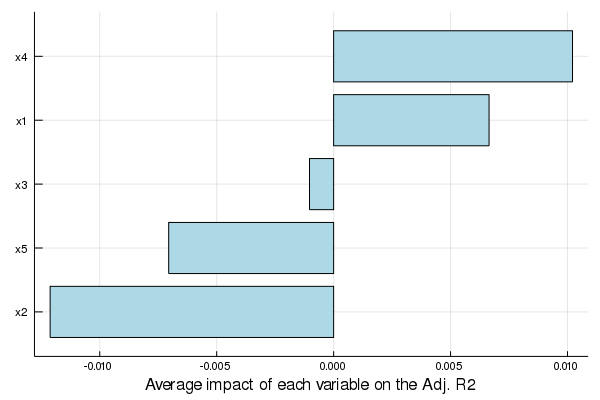
\includegraphics[scale=0.6]{cov_relevance.png}
\end{figure}

In this figure it is shown that potential covariates included in the general unrrestricted model of the all-subset-regression algorithm display singnificant differences in terms of the user selected information criteria. For each explanatory variable information criteria gains were obtained as the differece between averages information criteria obtained from models which includes and excludes that covariate. Available statistics suggests that there   explanatory  that improved model accuracy.  or }} helps to increase up to a \% the user selected information criteria. On the contrary, there    that have a deleterious impact on model accuracy. This is specially true for , which seems to decrease up to a \% the user selected information criteria}}


\addcontentsline{toc}{section}{References} 
\bibliographystyle{unsrt}  
\begin{thebibliography}{1}

\bibitem{gsreg2019}
Panigo D., Glüzmann P., Mocskos, E., Mauri Ungaro, A., Mari, V., and Monzón, N. (2019). \textit{GlobalSearchRegression.jl: Building bridges between Machine Learning and Econometrics in Fat-Data scenarios}.Paper presented at JuliaCon2019, Baltimore-MD, United States.

\bibitem{hassani2007}
Hassani H. (2007). \textit{Singular Spectrum Analysis: Methodology and Comparison}. Journal of Data Science, 5, 239-257.

\bibitem{lehmann2013}
Lehmann, R. (2013). \textit{3 sigma-rule for outlier detection from the viewpoint of geodetic adjustment}. Journal of Surveying Engineering, 139(4), 157-165.

\bibitem{tibshirani1996}
Tibshirani, R. (1996). \textit{Regression shrinkage and selection via the lasso}. Journal of the Royal Statistical Society: Series B (Methodological), 58(1), 267-288.

\bibitem{chandrashekar2014}
Chandrashekar, G., and Sahin, F. (2014). \textit{A survey on feature selection methods}. Computers & Electrical Engineering, 40(1), 16-28.

\bibitem{gluzmann2015}
Gluzmann, P., and Panigo, D. (2015). \textit{Global search regression: A new automatic model-selection technique for cross-section, time-series, and panel-data regressions.} The Stata Journal, 15(2), 325-349.

\bibitem{arlot2010}
Arlot, S., and Celisse, A. (2010).\textit{A survey of cross-validation procedures for model selection}. Statistics surveys, 4, 40-79.

\bibitem{jung2015}
Jung, Y., and Hu, J. (2015). \textit{A K-fold averaging cross-validation procedure}. Journal of nonparametric statistics, 27(2), 167-179.

\bibitem{bergmeir2012}
Bergmeir, C., and Benítez, J. M. (2012). \textit{On the use of cross-validation for time series predictor evaluation}. Information Sciences, 191, 192-213.

\bibitem{bergmeir2018}
Bergmeir, C., Hyndman, R. J., and Koo, B. (2018). \textit{A note on the validity of cross-validation for evaluating autoregressive time series prediction}. Computational Statistics & Data Analysis, 120, 70-83.

\bibitem{hyndman2013}
Hyndman, R. J., and Athanasopoulos, G. (2013). Measuring forecast accuracy. Gilliland M, Tashman L, Sglavo U. Business forecasting: practical problems and solutions, 177-84.

\end{thebibliography}


\end{document}